\chapter{Design}

\section{Goals}
Technical objectives I aim to acheive
\begin{enumerate}
    \item Implement a efficient historical Bitcoin data extractor for storage in a database - designing the historical collection process to run over several hours, rather than several weeks, as in previous work \cite{RefWorks:doc:5c98e031e4b068320632cef2}.
    \item Implement a mechanism for writing new Bitcoin data to the database upon new blocks being confirmed by the network.
    \item Implement a system for fetching historical Bitcoin price data for each Block at the time it was mined.
    \item Implement a system for building a dataset which maps bitcoin addresses to known entities of the bitcoin networks (e.g. exchanges, gambling sites, other services etc.) and generate relationships to write to the database for these mappings.
    \item Implement an API which interfaces the database
    \item \todo{Fill this in}
\end{enumerate}

\section{At my Disposal} 

\subsection{Hardware}
The primary hardware requirement is a very large amount of SSD storage. SSD storage can provide us with fast write speeds required to churn through the huge volume of data that must be written to Neo4J for the initial database setup.
\\\\
The hardware the department has at its disposal is a machine named 'satoshi' and has the following specification:
\begin{itemize}
    \item \textbf{Processor}: 24 core AMD EPYC 7401 
    \item \textbf{Memory}: \todo{get machine specification}
\end{itemize}
However, I will be using a VM on this machine, allocated a generous amount of the resource available, but of course not all. Additionally, I have root access on this VM so I am not limited to the software I am able to install on it. 
\\\\
My VM has the following resource allocated to it (initially):
\begin{itemize}
    \item \textbf{Cores}: 16 cores 
    \item \textbf{Memory}: 16GB
    \item \textbf{Storage}: $\sim$5TB SSD Free
\end{itemize}

\subsection{Bitcoin Full Node}
There already exists a Bitcoin Full Node running in a persistent Docker container which I am able to connect to. Using the RPC interface provided by Bitcoin Core, I am able to poll and fetch Bitcoin data. 

\section{Technology Assessment}


\subsection{Graph Databases}
A graph database is a type of database where the relations between data are of equal importance to the data itself. Data does not need to be constricted to a pre-defined structure; rather it is stored using a flexible combination of nodes and relationships between them. 

\subsubsection{Why use a Graph DB for storing Bitcoin?}
Graph DB's provide efficient traversing of nodes; allowing million of connections to be traversed per second per core \cite{RefWorks:doc:5c98f0c6e4b00cbb4da393d8}. Scaling independently to the size of the data-set, a graph database is excellently suited for storing the vast, complex data-set constituting the Bitcoin Blockchain. 

\subsubsection{Neo4J}
Neo4J is an open-source, NoSQL graph-database providing ACID compliant transactions.



\section{Database Population Approach}
There exist several approaches to populating a database with the Bitcoin Blockchain; since we are working with a dataset of such vast scale, it is certainly a worthwhile investment at this stage to analyse the merits of each approach and decide which will be most suitable. Otherwise, taking a naive approach would risk a very time consuming, and potentially fragile process, which may hamper progression with subsequent stages of this project. 

\subsubsection{Overview of Approaches}
\begin{enumerate}
    \item Running a full Bitcoin node [see \ref{background-nodes}]. Download the entire Blockchain, use a custom script to parse the files write the data to the database. Keep database up to date using long polling / \gls{rpc}. 
    \item Leverage some of the work done by a previous project in the Department of Computing at Imperial for Blockchain health monitoring \cite{RefWorks:doc:5c6bd151e4b041254f892045}. The initial population of the database would require re-running the RPC approach used in this project, then creating a Kafka consumer to keep the database up to date. 
    \item Combining the two approaches of above: create a custom script for initial database population, but then use the Bitcoin health service for keeping the database up to date. 
\end{enumerate}

\subsection{Previous Work}\label{design-db-previous-work}
\subsubsection{Bitcoin to Neo4J Tool : Open Source Project}
There exists an open source tool, built by the author of the website \url{learnmeabitcoin.com}, which populates a Neo4J database with the entire Bitcoin Blockchain \cite{RefWorks:doc:5c98e031e4b068320632cef2}. This tool requires a full Bitcoin node to be run in order to have the .dat files stored locally; the tool will parse the .dat files and write them using Cypher queries to the Neo4J database. This approach has the advantage that it is a respected approach in the community to this task and has been cited a number of times by those seeking to achieve the same goal \cite{RefWorks:doc:5c98e0cde4b044512c0b8641}; however, the tool will take several weeks (apparently 60+ days) to complete the import. 

\subsubsection{Max Baylis : Imperial MSc Project 2018}
Max undertook a project titled 'Blockchain Data Analytics and Health Monitoring' within the Department of Computing at Imperial \cite{RefWorks:doc:5c6bd151e4b041254f892045} which involved bulk extracting data from several blockchains and writing that data to a MongoDB database. He additionally used Kafka for providing clients with the most recent blockchain updates which complimented the historical data in the database. This data was used for providing blockchain analytics in a web based environment \cite{RefWorks:doc:5c6bd151e4b041254f892045}. 

\subsubsection{TokenAnalyst : Medium Blog}
TokenAnalyst wrote a blog article on Medium with the title 'How to load Bitcoin to Neo4J in a day' \cite{RefWorks:doc:5c98e0cde4b044512c0b8641}. They describe their process of using RPC to fetch the data, writing the data to a 'data lake' in a compressed Arvo format, generating CSV's from the compressed files and feeding them to Neo4J's bulk import tool. Similar to Max's work, they then use Kafka for steaming the most recent Bitcoin data to a tool which writes it to Neo4J to keep the database up to date. 

\subsubsection{Blockchain2graph : Open Source Project}
A company Blockchain Inspector who are 'using Artificial Intelligence to fight fraud in the Blockchain' have open-sourced a tool they use with the claim that it extracts Bitcoin data and writes it to a Neo4J database \cite{RefWorks:doc:5cac6184e4b01c076c63e173}.

\subsubsection{Analysis of previous work}
TokenAnalyst's approach seems to best describe the ideal situation for this project; a efficient bulk import into Neo4J and a mechanism for keeping the database up to date. There exists no open source implementation for their work, only a high level description of what they did in their blog post. Max's work, however, is available to me and his work in fetching data using RPC could prove useful to my project. The Bitcoin to Neo4J tool would not be a feasible approach and can be immediately ruled out due to the time requirement of several weeks for the tool to complete; this would not be acceptable for the timescale of this project. As for Blockchain Inspector's open-source solution, upon inspection of the code, it seems the bulk import process relies on an existing database containing the entire Bitcoin Blockchain, and therefore seems to be more of a tool to migrate from a traditional database to a relational one (Neo4J). It is therefore not very applicable to my work, creating an intermediate database storing the Bitcoin Blockchain for the bulk import would be unnecessary and expensive. 

\subsection{Running a full node}
Running a full node (Bitcoin Core) would download the entire Bitcoin Blockchain to the current tip; the blockchain is currently at ~197GB\cite{RefWorks:doc:5c6ab1a3e4b05e3aaec0ffc8} in size and would consume a considerable amount of storage, and time to download). This would provide the .dat files containing all Bitcoin Blockchain data to the date of download. 

\subsection{High Level Plan}
There were two main phases to populating the database. First, historic data population. Then the second phase will be keeping the database up to date with new data as it arrives. Taking inspiration from TokenAnalyst's approach, and extending the existing work by Max Baylis as described in section \ref{design-db-previous-work}, I created a tool to succesfully download the entire Bitcoin Blockchain, write it to a Neo4J database and keep it up to date in just a day.

\subsection{Historic Data Population}
Max's implementation uses WebFlux to create parallel streams of data fetched using RPC and writes it to MongoDB; I adapted this work to divert the data into a CSV format suitable for importing into Neo4J. The steps below describe the steps taken to successfully build CSV files for the entire Bitcoin Blockchain. 

\begin{itemize}
    \item Introduced a new API endpoint for Admin usage. The new endpoint was named \texttt{extractBitcoinToNeo4j}. This accepted two arguments as path variables, \texttt{fromHeight} and \texttt{toHeight} which are to be used to define the range of blocks to fetch data from. 
    \item Using the parameters \texttt{fromHeight} and \texttt{toHeight}, I then generate a Flux stream which uses RPC to invoke the method \texttt{getBlockHash} on a \textit{bitcoind} instance running in a container on the same machine. 
    \item The Flux stream of block hashes are then mapped to the actual block data using flux's \texttt{flatMap} operation and by invoking the method \texttt{getBlock}, passing it the block hash from the previous step. 
    \item The block data is retrieved and deserialized to an intermediary representation in Java. Each block will then be written to a CSV file in the format required for an import into Neo4J. 
    \item The retrieval of a single block will then kick off the process of fetching transactions; the Flux of blocks will be mapped to individual transactions by fetching each of the transaction ID's in the block and again using RPC to invoke the \texttt{getrawtransaction} on the \textit{bitcoind} instance in order to fetch all the data for each transaction. 
    \item Each retrieved transaction will be written to CSV, in addition to writing the relationships between transactions, blocks and outputs to their own CSV files. 
\end{itemize}

\begin{figure}[h!]
  \centering
  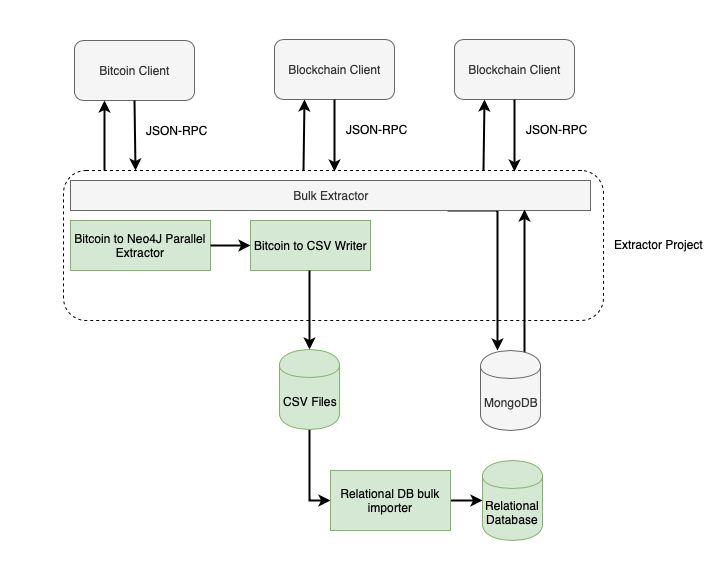
\includegraphics[width = 15cm]{./figures/adding-bitcoin-extractor-diagram}\\[0.5cm] 
  \caption{A architecture diagram displaying the new components (in green) I introduced to Max's Blockchain Health project while implementing Bitcoin to Neo4J historic data population}
  \label{fig:neo4j-layout}
\end{figure}


\subsection{Data Format}

\subsubsection{Data Nodes}
\begin{itemize}
    \item \texttt{BLOCK} : A Bitcoin block, unique id being the block hash. 
    \item \texttt{TRANSACTION} : A Bitcoin transaction, unique id the txid property
    \item \texttt{OUTPUT} : A transaction output, unique id the txid property concatenated with the outputs index in the transaction
    \item \texttt{ADDRESS} : A Bitcoin public address, unique id the public address itself
\end{itemize}

\subsubsection{Relationships}
I created several types of relationships to exist between nodes in Neo4J. The relationships can be seen in a visual representation below in figure \ref{fig:neo4j-layout}.
\begin{itemize}
    \item \texttt{CHAINED\_FROM} Exists between two blocks; represents the relationship between a block and it's parent block. 
    \item \texttt{MINED\_IN} Exists beween a transaction and a block. Represents the relationship between a transaction and the block it was mined in. 
    \item \texttt{LOCKED\_TO} Exists between a transaction output and an address. Represents the relationship between an output, and who it can be spent by. 
    \item \texttt{INPUTS} Exists between a transaction output and a transaction. Describes the relationship between an output and the transaction it later funds. 
    \item \texttt{OUTPUTS} Exists between a transaction and a transaction output. Shows the relationship between a transaction and the new outputs it generates. 
    \item \texttt{COINBASE} Exists between a transaction output and a block. Represents the special type of input to a transaction which generates new bitcoin, and is associated with a block as it was the miners reward for successfully mining the block. 
\end{itemize}

\begin{figure}[h!]
  \centering
  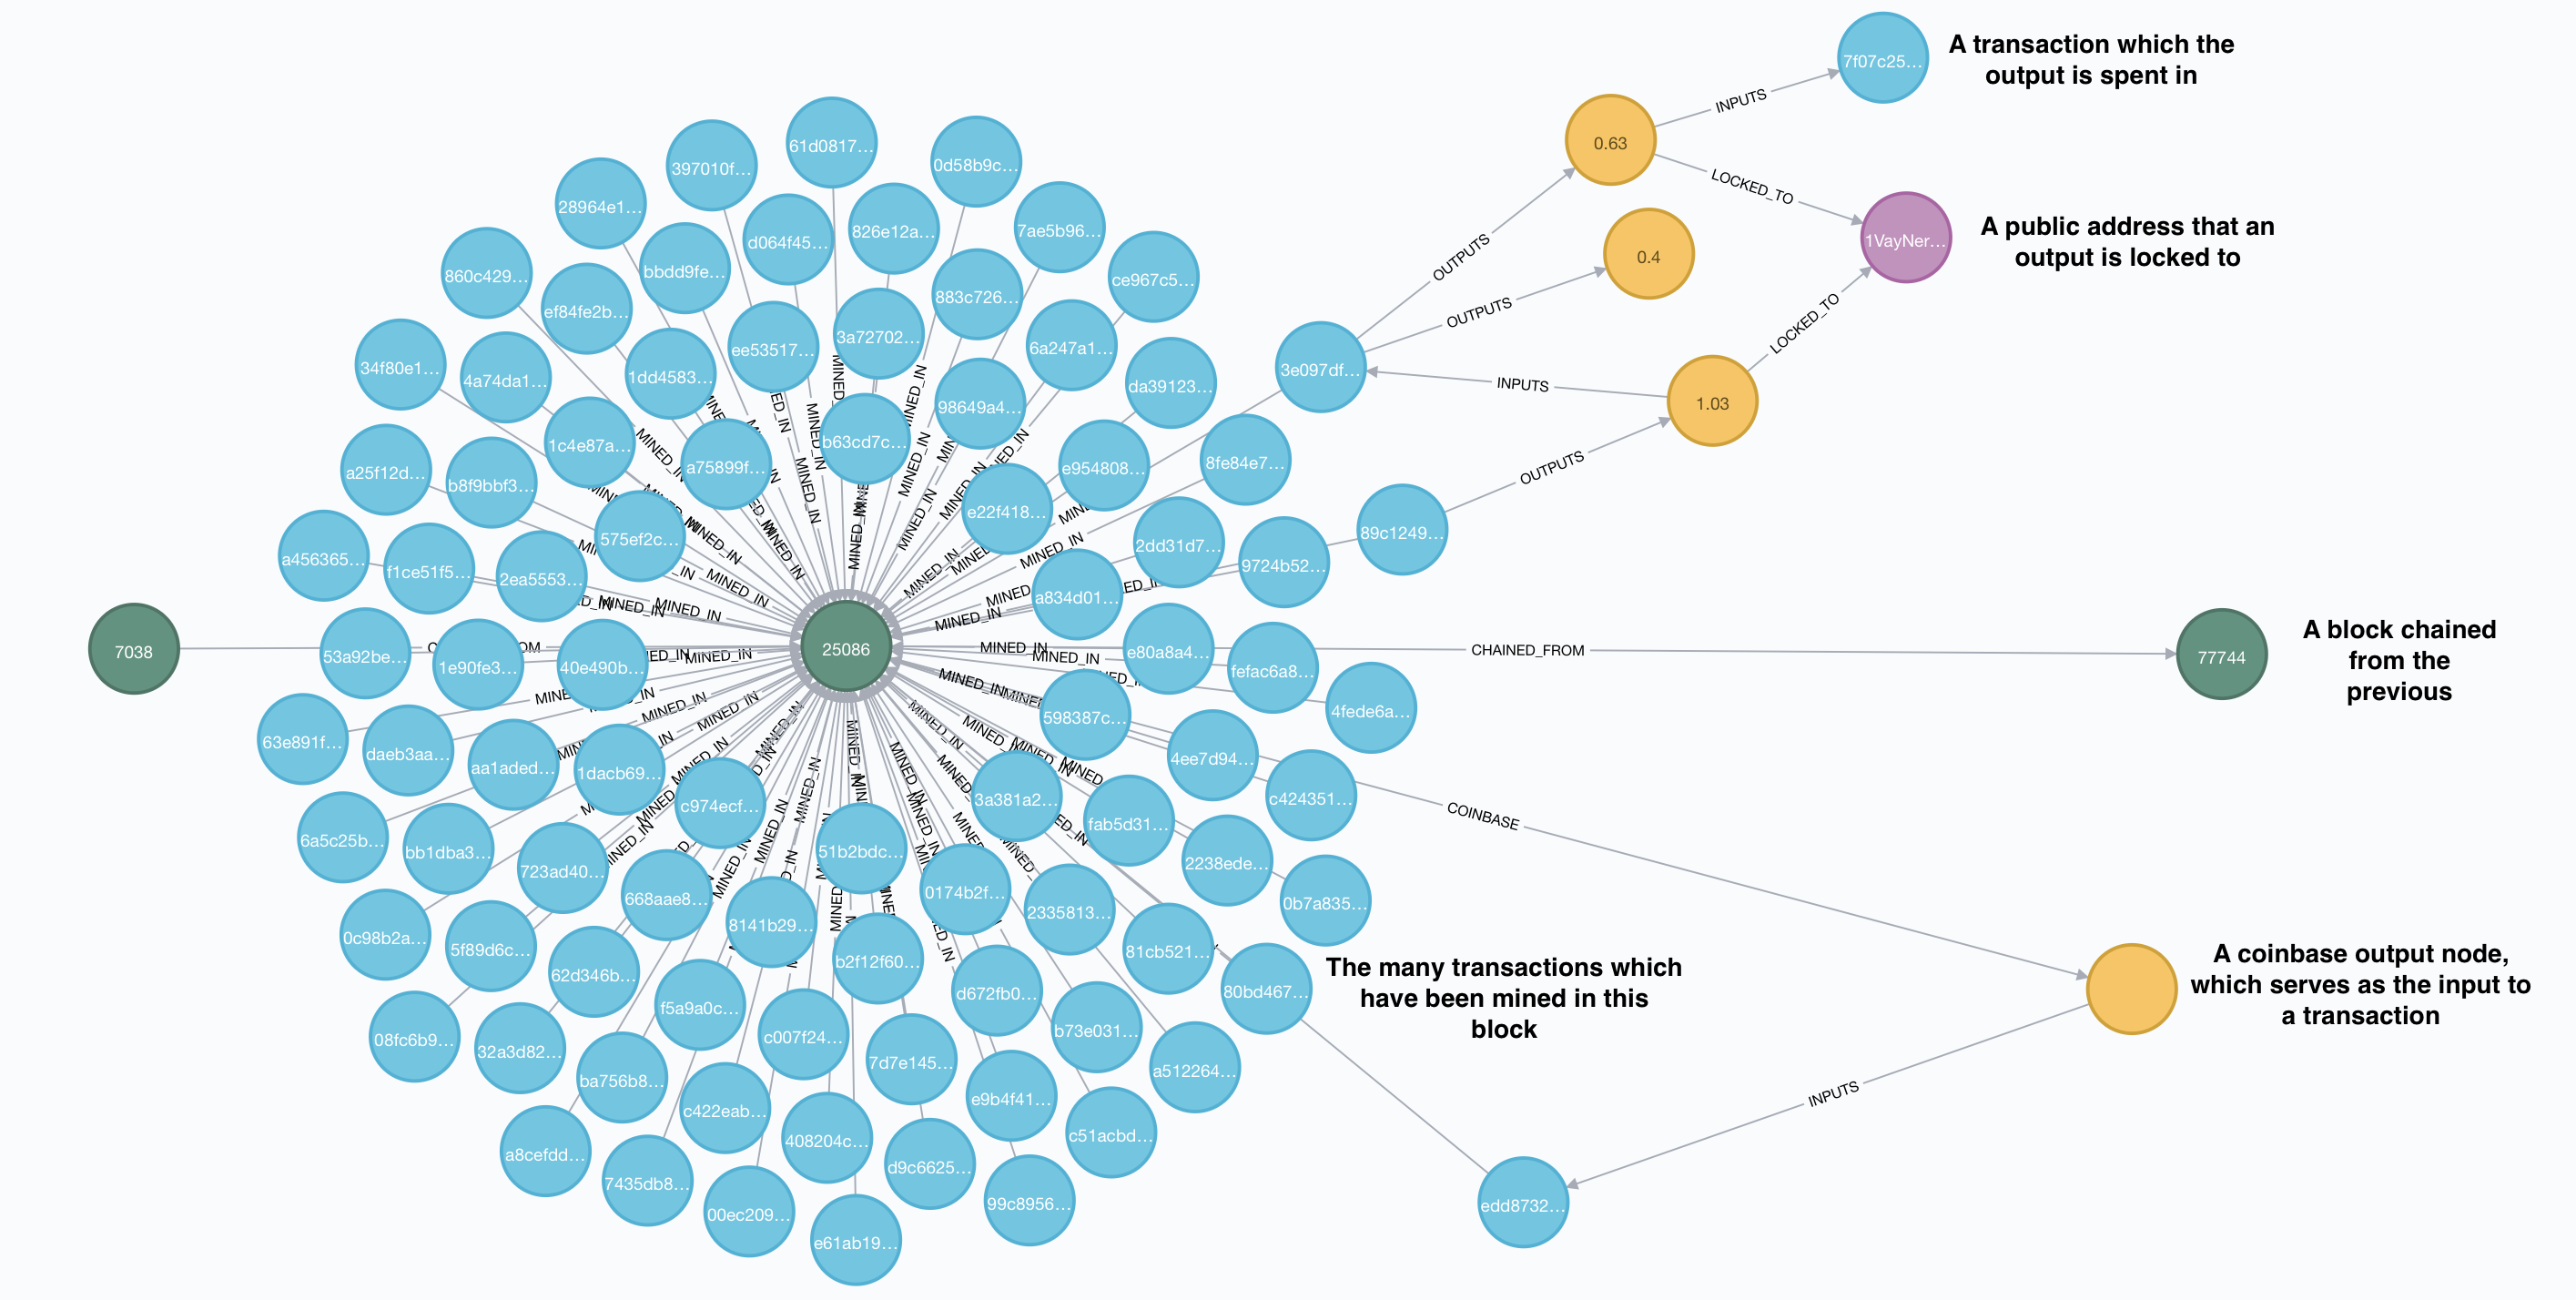
\includegraphics[width = 15cm]{./figures/neo4j-annotated}\\[0.5cm] 
  \caption{The nodes and relationships as visualised using the Neo4J Web UI}
  \label{fig:neo4j-layout}
\end{figure}

\subsection{Challenges \& Solutions:}
\subsubsection{Efficiency}
With multiple cores at my disposal, it would only be logical to try and distribute the workload across the cores. Fortunately, WebFlux conveniently provides functionality to do this; by adding \texttt{.parallel(n)} to my Flux stream, the workload is divided up into \texttt{n} rails. Then subsequently applying the \texttt{.runOn(Schedulers.parallel())} mapping, WebFlux is told to parallelise this work by running each rail on a separate core. 
\subsubsection{Job failure mitigation}
When an error from the client is received, possibly due to being overwhelmed with requests, it would be far from ideal for a single failure to cause the entire job to fail. Therefore I mitigated job failure by adding retry logic when requesting using the Reactive Client, so that failures will be handled by re-trying with a delay (the delay necessary to allow time for producer recovery in the case of being overwhelmed). Additionally, if an unexpected error occurs that I have not anticipated, the entire job may fail. Therefore, when performing the download, I ensured to do so in incremental batches. E.g I first download data for blocks 0-100,000 then 100,001-200,000 and so on. Therefore, if a failure does occur, progress from other blocks has been saved from previously successful runs and only the batch which failed needs to be re-run. 

\subsubsection{Writing concurrently from several threads}
Although the above parallelisation improves the efficiency of the overall download process, it introduced the problem of multiple threads writing to a single CSV file concurrently, which led to data in the CSV files being malformed where threads have written data chunks in an interleaving fashion. 
\\\\
\textbf{Fix interleaving writes with a lock:} Clearly each line in the file needs to be written atomically, so I introduced a lock that each thread must hold in order to perform a write to a CSV file. However, I quickly realised that this will create a significant bottleneck in the workflow and developed an alternative solution.
\\\\
\textbf{Fix interleaving writes with per thread files:} To enable parallel file writing and prevent the bottleneck of acquiring locks, I created a CSV file writer for each thread, for each data type. For example, the CSV file containing the block nodes will be named \texttt{block-data-thread-1.csv}, \texttt{block-data-thread-2.csv} and \texttt{block-data-thread-3.csv} etc. With this solution, each write can occur without risk of another thread also attempting to write, so the overhead of acquiring a lock for concurrent access is now redundant. \todo{Compare runs with and without}

\subsubsection{Duplicate Addresses}
While generating the CSV files, we fetch the outputs of a transaction an the addresses each output is locked to. Since while generating the CSV, there was no way of efficiently checking if we had already seen an address before, we simply had to write every address we see to the CSV file. When running the Neo4J bulk import job, we encounter an error as we attempt to define an address node twice. A solution considered was to use a flag \texttt{--ignore-duplicate-nodes} that can be used when invoking the bulk import tool. This would simply ignore any address nodes that have already been defined, solving our problem. However, as TokenAnalyst found in their work \cite{RefWorks:doc:5c98e0cde4b044512c0b8641}, the \texttt{--ignore-duplicate-nodes} flag massively slows down the import process, as Neo4J needs to check every single node to see if the one its adding already exists. Their solution, which I adopted, was to use GNU's \texttt{sort - u} command, which allows us to generate a new address CSV file with only the unique addresses. TokenAnalyst found this process to take around 30 minutes \cite{RefWorks:doc:5c98e0cde4b044512c0b8641}, and is therefore a good investment in speeding up the entire import process. 
\\\\
\textbf{Sanity checking the number of addresses: } For blocks 0-570,000, I used the \texttt{wc -l} command to count how many address entries that had been written to CSV (including all duplicates). This sum came to 1,052,218,849 entries. Performing the unique sorting operation, using the aforementioned \texttt{sort -u} command, which took a total time of 50 minutes 3 seconds,  I produced an address file containing only unique addresses, and again performed a count operation which came to 495,668,754 unique addresses.
\\\\
In order to sanity check this value, I used the data provided by blockchain.info; they provide a daily measurement of the number of \textbf{active} addresses in Bitcoin each day. Clearly, our figure will be the cumulative sum of this figure since the Genesis block. In order to easily calculate the expected number of unique addresses using their data, I used their functionality to export this data to CSV and performed a sum over this data. 
\\\\
The block at height 570,000 was mined on 3rd April 2019. The data from blockchain.com has a data point for the 30th of March 2019 

\subsection{Performing the Neo4J Import}
I am now at the stage where I have the entire Bitcoin Blockchain in CSV file representation, with the relationship between all nodes. I can now use Neo4J's bulk import tool, passing it the CSV files, header files and relationship data. 

\subsubsection{Bulk Import Tool}
Neo4J provides functionality for bulk importing data \cite{RefWorks:doc:5c6ab610e4b02c4a19ae3ed1}. A Neo4J blog describes an example use of this functionality: importing a  vast 66GB dataset from Stackoverflow into a new Neo4J database \cite{RefWorks:doc:5c6ab2bae4b08c9b85da964f}; however, this is less than a third the size of the Bitcoin blockchain (approximately 197GB at the beginning of January 2019 \cite{RefWorks:doc:5c6ab1a3e4b05e3aaec0ffc8}).
\\\\ 
The Stackoverflow import example shows usage of Cypher features for improving the efficiency of bulk imports, such as 'constraints', 'indexes', 'distinct'  in order to make the import more efficient. Another useful feature is periodicc commit' which allows the transaction state to be intermittently committed to storage, and the memory Neo4J is using to hold this state to be flushed. 
\\\\
The import tool is designed to take advantage of the hardware at it's disposal; ideal for our use-case where we have a large amount of SSD and processing power available, and we simply need to ensure we can take full advantage of it. The Stackoverflow import took just over 3 minutes to complete \cite{RefWorks:doc:5c6ab2bae4b08c9b85da964f}. 

\section{Fetching Historical Price Data}
A planned feature of the system is to be able to view the value of Bitcoin transaction outputs in several fiat currencies at the time the transaction occurred. The fiat currencies to be used are GBP, USD and EUR. In order to achieve this functionality, the historical price index for Bitcoin must be collected and stored for the entire time spanning from the infancy of Bitcoin to the present day. 

\subsection{Collecting the price data}
Fortunately, CoinDesk have an API providing the historical Bitcoin price index data from late July 2010 onwards \cite{RefWorks:doc:5cacd8cbe4b092e311880f2b}. The API can fetch the daily price index for each day in a provided date range, with conversions into the desired fiat currency. 

\subsection{Storing the price data}
Since the historical price data retrieved from CoinDesk is at the granularity of one data point per day, and a block in bitcoin mined approximately every 10 minutes, it would be appropriate for the price data to be stored with each block in the database. Storing the data with each transaction output would not provide any additional value, and would lead us to encounter a greater storage overhead and computational resource in associating the price data with every transaction output in Bitcoin. Since each output is associated with a transaction as an output (the \texttt{OUTPUT} relationship), and each transaction associated with the block it was mined in (the \texttt{MINED\_IN} relationship), we can easily find the price index data for an output in just a couple of hops. 
\\\\
The price index data for each block can therefore be fetched using the CoinDesk API and added to the CSV file containing all blocks. 

\subsection{Implementing historical price collector}
Using Python3, I created a program to accept CSV file names as input (or a regex for matching files), read through each line of the CSV (representing a single block) and write a new output line with each row (block) augmented with the price data at the time the block was mined in GBP, USD and EUR. 
\\\\
Since at the time of writing, the current Bitcoin block height was $>$ 570,000, and it would not be ideal to make a price index request for each block, 3 times over for each currency. Therefore, the program first checks a local cache to see if the price data is already available for a particular date. If not, it performs a fetch which collects the data for that date and the following 300 days and populates the cache. We therefore reduce the total number of requests made, and the overhead associated with making each request, while also avoid making the request excessively large by collecting data for a much greater date range. For example, fetching 1000 days would lead to less requests being made for blocks covering several years, but an unnecessary overhead when fetching data for blocks covering only 100 days.

\section{Public Address Entity Tagging}
walletexplorer.com hosts a wealth of data mapping entities (e.g exchanges, pools, services etc) to the public addresses they are known to operate under \cite{RefWorks:doc:5c4b26f3e4b0ea619646d513}. This data would be extremely valuable to the task of clustering addresses by the entities they belong to. 

\subsection{Fetching the data}\label{design:fetch-entity-data}
walletexplorer.com do not provide any functionality for users to download the data they serve. The data can only be viewed by navigating to each wallet, then their addresses, then through a series of paginated tables providing the addresses for that entity. 
\\\\
My solution to this problem was to build a web scraping application which navigates the site and builds a mapping for each wallet (entity) to all of it's addresses, which can then be written to some output file for mapping against my stored bitcoin data at a later stage. 

\subsubsection{Building the scraper}
I used a popular open-source web-scraping framework scrapy for building my scraper application. I simply generate a new 'spider' for my scraping operation by extending the frameworks 'CrawlSpider' class. In this class, I define the bounds of the crawl, and methods to parse and extract the data on each page it visits. For example, I created rules to allow the cralwler to navigate to links with 'addresses' in the URL and then defined how to extract the wallet name,  each of the addresses from the table and how to follow links to paginate the table in order to view all addresses for that wallet. 
\\\\
However, when I ran my scraper application, I continuously received 403 (Forbidden) error responses for the majority of my requests.  Through investigation, I discovered the likely cause of this was due to anti-scraping measures many websites employ. In order to circumvent these anti-scraping measures, I experimented with a number of approaches recommended by scrapys documentation titled 'Avoid getting banned'; these included rotating user agents, disabling cookies, use download delays or use a pool of rotating IP's. 
\\\\
\textbf{Implementing delays:} This approach worked; I was able to visit many pages without being served a 403 response as before, however this took a very long time. A delay of more than 2 seconds was required to enable to delay solution to work; this would therefore take an infeasible amount of time to scrape the thousands of pages containing the required data on the walletexplorer site. 
\\\\
\textbf{Using rotating proxies:} I integrated into my scraper project scrapoxy which allows me to hide my scraper behind a cloud provider (in this isntance AWS). Scrapoxy creates a pool of proxies and routes all requests through the pool of proxies. I configued scrapoxy to use my personal Amazon EC2 account, and was able to scale up to 20 EC2 instances when performing the scraping (to enable greater concurrency, but limited at 20 because my account is restricted to 20 instances).  Through trial and error, I was also able to configure the number of concurrent requests per proxy to 5, which further maximises concurrency without encountering errors due to anti-scraping measures. 
\\\\
\textbf{Results}: Using 20 EC2 instances, the scrape completed on 14-04-2019 at 10:07:42 successfully after 1 day, 19 hours and 12 minutes and received 240,411 HTTP responses. This amounted to generating a 920MB data file containing entity to address mappings. Due to the wallet addresses existing over several pages and the asynchronous nature of scraping each page, a wallet may have many entries in the output file JSON. For example, the resulting format will be:

\begin{lstlisting}
[
{"wallet": "wallet1", "addresses": ["add1", "add2"]},
{"wallet": "wallet2", "addresses": ["add3"]},
{"wallet": "wallet1", "addresses": ["add4", "add5"]}
]
\end{lstlisting}

whereas we would like the desired format to be of the format:

\begin{lstlisting}
{
"wallet1": ["add1", "add2", "add4", "add5],
"wallet2": ["add3"]
}
\end{lstlisting}
Thankfully the size of the input file was still small enough to load into memory, making this transformation simpler. I created a simple script which iterated through the input file and generated a new dictionary containing wallet names as unique keys and concatenated lists of addresses from each entry matching the wallet name. I then wrote this out to in JSON format to a new file. 


\subsection{Tagging addresses with entity data}
\subsubsection{Augmenting the data model}
\begin{itemize}
    \item new entity node for each wallet?
    \item do we want types of entties separate?
    \item need to read through every address, match it against candidate addresses,  then find the entity it maps to, and create a new relationship entry for  address-> entity
\end{itemize}

\subsubsection{Extended data model}
The first thing to consider was how to represent that an address is controlled by a known entity. I achieved this by extending the existing Neo4J data model with a new node type for each known entity. I then created a new relationship \texttt{HAS\_ENTITY} which exists between entities and the addresses they are known to control (learnt from the data in the previous step \ref{design:fetch-entity-data}) and can be seen in figure \ref{fig:neo4j-has-entity} 

\begin{figure}[h!]
  \centering
  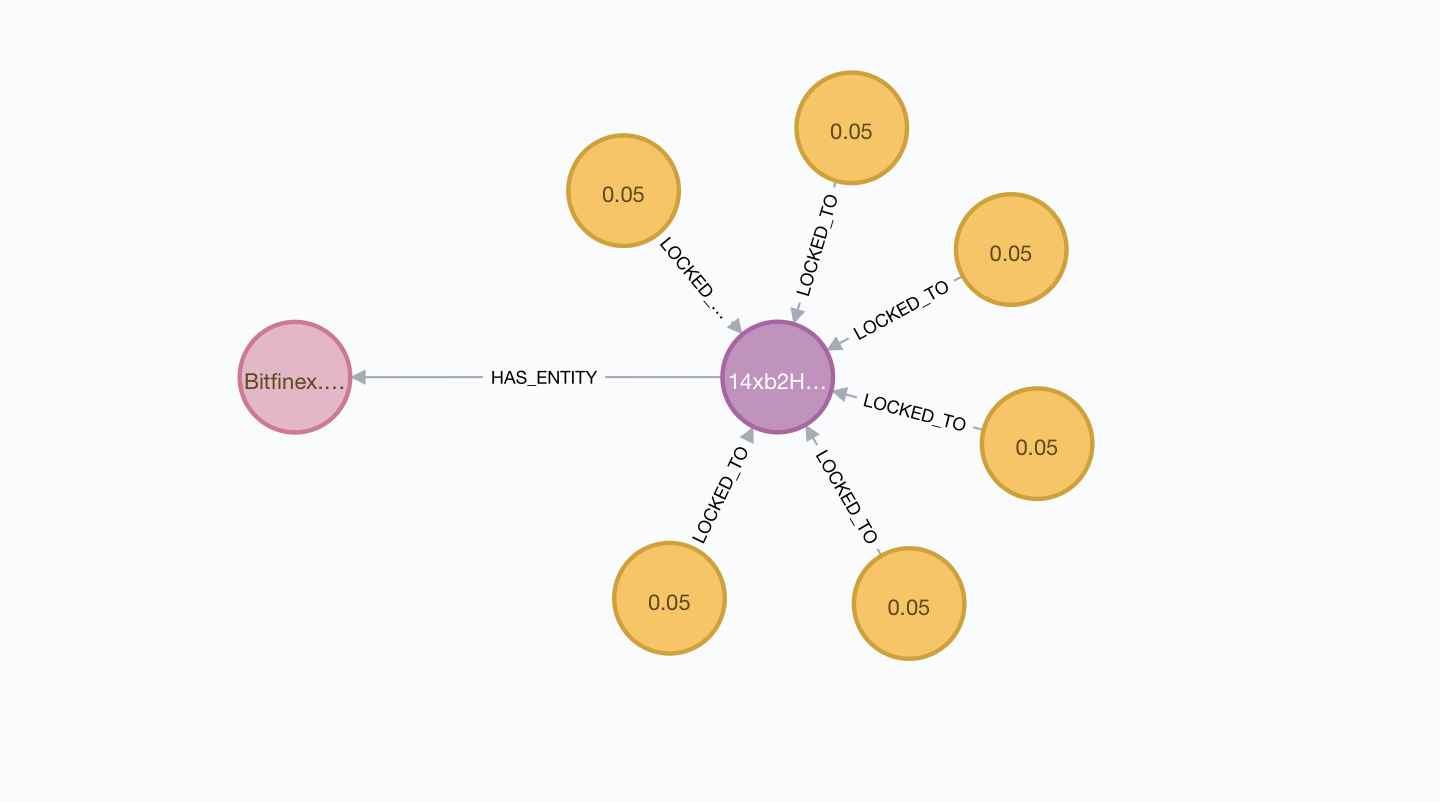
\includegraphics[width = 15cm]{./figures/has-entity-relationship}\\[0.5cm] 
  \caption{The new \texttt{HAS\_ENTITY} relationship visualised between a new Entity node and a bitcoin address.}
  \label{fig:neo4j-has-entity}
\end{figure}

\subsubsection{Performing the address matching} 
From step \ref{design:fetch-entity-data} we have a JSON mapping each entity type to a list of addresses. From importing the Bitcoin Blockchain into CSV format, and de-duplicating addresses, we have a CSV containing all distinct addresses to have ever been seen on the chain. I now have the task of creating a new \texttt{HAS\_ENTITY} relationship for each address in the CSV that occurs in the entity mapping JSON file. If I were to take a naive approach here, where I would compare each address from the blockchain against each address I have a mapping for, I would have an algorithm which performs $\mathcal{O}(nm)$ address matches, where $n$ is the number of addresses found on the blockchain and $m$ the number of addresses I have an entity mapping for. 
\\\\
A better approach would be to use a Trie data structure. The Trie data structure will be a more efficient method of storing the entity mapping address data since it only need to store once the inevitable common prefix's of the millions of addresses. The primary benefit, though, is for performing the address matching. For each address in the blockchain, we only need to walk at most the height of the tree once, so we only require $\mathcal{O}(n)$ address matches. I was able to simply implement this approach using Tries by using Google's pygtrie library. 

\subsection{Performing the bulk historical import}

\subsubsection{Invoking the import job}
I created a script to wrap the execution of the import job, providing the benefits of version control and reproducibility. This script first uses globbing to build the list of input files for each type of node and relationship. It then invokes the import command as shown below. Some additional arguments were \textt{--max-memory} to override the default 90\% memory usage to use slightly more. The argument \textt{--ignore-missing-nodes} was to prevent a long job failing simply due to a single relationship referring to a non existing node, and to rely on these bad relationships being reported to the file as defined by the \textt{--report-file} option for manual investigation. 
\\\\
\begin{lstlisting}[language=Bash]
$1/bin/neo4j-admin import 
  --nodes:ADDRESS $address_files_all
  --nodes:BLOCK $block_files_all
  --nodes:COINBASE $coinbase_files_all
  --node:OUTPUT $output_files_all
  --nodes:TRANSACTION $transaction_files_all 
  --nodes:ENTITY $entity_files_all
  --relationships:CHAINED_FROM $relation_chained_from_files 
  --relationships:COINBASE $relation_coinbase_files 
  --relationships:INPUTS $relation_inputs_files 
  --relationships:LOCKED_TO $relation_locked_to_files 
  --relationships:MINED_IN $relation_mined_in_files 
  --relationships:OUTPUTS $relation_outputs_files 
  --max-memory 95% 
  --ignore-missing-nodes true 
  --report-file "neo4j-import-debug-report.log" 
\end{lstlisting}

\subsubsection{Challenges}
While attempting to perform the bulk import, I encountered an issue where the import job would fail with no output other than message that the process was killed. This occurred deterministic at around 28\% progress into the graph node creation process. After investigation, I found that this issue was being caused by Neo4J running out of available memory; I rectified this by partitioning a much larger amount of Swap memory for the VM. This allowed the import tool to store information in virtual memory once physical memory had been exhausted. 

\subsubsection{Result}
The import operation for the first 570,000 Bitcoin Blocks completed in 5 hours, 32 minutes and 54 seconds. The operation consumed 22.96GB of memory and created 1.964 billion nodes, 3.52 billion relationships and 3.03 billion properties. There were no errors or bad relationships reported. 

\section{Building a REST API to interface Neo4J}

\subsection{Technology}
Java, Spring Data, Spring Boot

\subsection{Implementation}

\begin{itemize}
    \item build model classes to represent the nodes, used @Relationship annotation to fetch nodes a 1 hop relationship away
    \item had to use jsonignoreentities to represent infinite recursion fetching entities that include eachother through the relationship property 
    \item build a rest controller which exposes an api to fetch each type of node given their id
    
\end{itemize}


\section{Building the UI} 
\begin{itemize}
    \item why angular? some familiarity with it from previous projects. supports data binding which is important for this application. has tools like angular cli to quickly scaffold out project which reduces setup time. well supported in the front end community. 
    \item uses angular CLI to scaffold out the project
    \item uses D3 for drawing svg nodes and links in a force directed graph 
    \item uses RXJS for asynchronous http calls and implementing publish/subscribe patterns for communicating data across several views (e.g search results are pushed to a data observable which is listened to by the investigation view which renders new nodes whenever new data arrives) 
    \item stage 1: search by address. node rendering, relation expansions
    \item stage 2: path finding between addresses
    
    
\end{itemize}